\subsection{Facilities \& Equipment}
\subsubsection{Equipment}
\textbf{QNAP}\\
Our sponsor has access to a device called a QNAP. A QNAP acts as a local storage device but also as a remote server when needed. This device is useful for our project because it gives us access to a sort of private server option for our users, if they would prefer not to use a OneDrive service or something similar. In using a QNAP or other private device, the users can specify files and folders for others to access and provide those access rights to our service for others to use. The QNAP is also handy because it provides a built in interface for users to tap into and easily find the files being offered by the provider.\\\\
\textbf{Microphones}\\
Some important equipment used by the researchers in the field of soundscape ecology include microphones. Our sponsor in particular uses a Wildlife Acoustics SM4 model along with the Wildlife Acoustics Song Meter device.\par
The Song Meter is considered the smallest and lightest dual channel acoustic recorder available\cite{songmeter}. The microphones record raw sound and store them in uncompressed .wav files. These .wav files can then be used by programs like ours to calculate the indices mentioned for analysis by researchers.\par
Our sponsor\textquotesingle s strategy is to place these microphones in multiple places in the environment being tested, to get a better understanding of the impact of sound on the ecosystem. In doing this, we can hear more of the sounds of the ecosystem and provide better index analysis.\par

\subsubsection{Facilities}
\textbf{UCF Arboretum}\\
The UCF arboretum was created in 1983 as a place for students and faculty to learn about ecology and work with the environment. The arboretum acts as a research area on campus for identifying plants and the local wildlife\cite{ucfarboretum}. This eighty acre span of land is home to hundreds of species of plants and animals, including vulnerable species like the Gopher Tortoise.\cite{pegasus}\par
Over the past year, our sponsor, Dr. Beever, has been conducting research in the arboretum and surrounding areas to gain a better understanding of the impact of humans on the local ecosystem using the Wildlife Acosutic microphones. One interesting segment of this research is a series of recordings made of Hurricane Irma during the 2017 hurricane season. With sustained wind speeds in the Orlando area during this hurricane reaching 59 mph (95 km/h),\cite{irmaspeed} the potential insights found from possible biophony within the recordings may prove to be intriguing.\\\\
\textbf{Central Florida Zoo}\\
Originally founded as the Sanford Zoo in 1923, the Central Florida Zoo has since become host to over 400 animals. It has since adopted a mission which, among other tenets, includes \enquote{contributing globally to the conservation and preservation of wildlife.}\cite{aboutzoo}\par
\begin{center}
	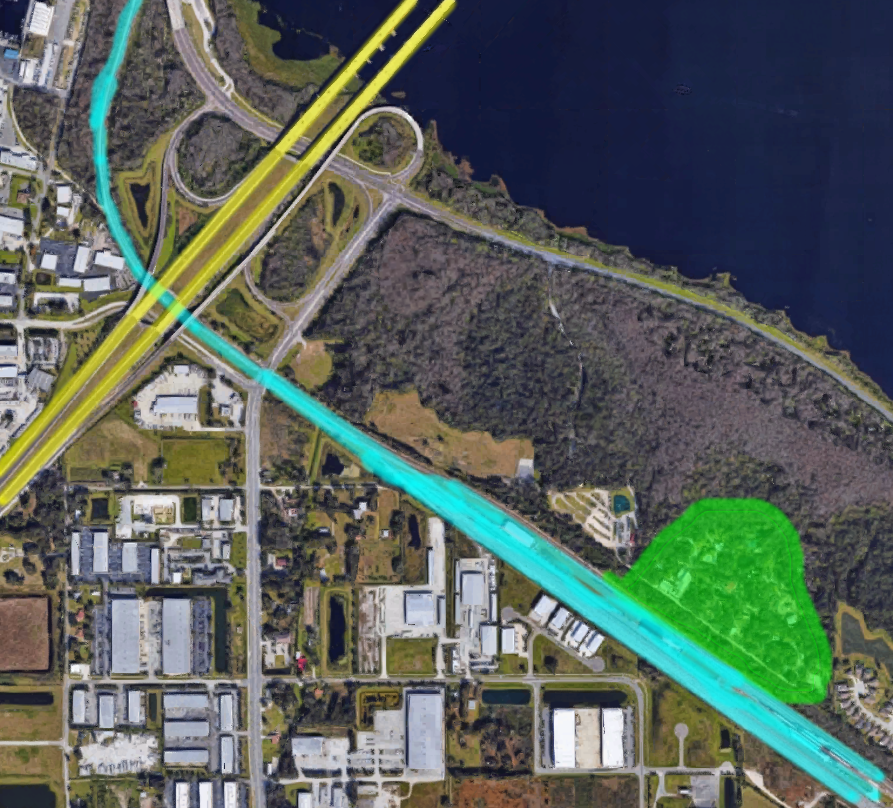
\includegraphics[width=\textwidth]{ZooMap}
\end{center}
In the past year, Dr. Beever obtained permission from the zoo (green) to place several of his microphones within the giraffe enclosure. With the enclosure only steps away from a Class I railway (blue) and about a mile away from Interstate 4 (yellow), he was curious to see how these massive sources of anthrophony could affect the biophony produced by the giraffes and, consequently, their general well being.
